
%% Essa classe foi adaptada do formato de conferências da ACM
%\documentclass[sigconf, review, anonymous]{educomp}

%Na versão final remover as tags review e anonymous
\documentclass[sigconf, review]{educomp}

\renewcommand\refname{Referências}

%% Não altere essas informações. Elas serão enviadas aos autores após ao aceite no ato da publicação dos anais.

\copyrightyear{2022}
\acmYear{2022}
\setcopyright{sbcpt} %%% Para artigos escritos em inglês, troque para sbcen
\acmConference[EduComp'22]{Simpósio Brasileiro de Educação em Computação}{Abril 25-29, 2022}{Feira de Santana, Bahia, Brasil (On-line)}
\acmBooktitle{Simpósio Brasileiro de Educação em Computação (EduComp '22), Abril 25-29, 2022, Feira de Santana, Bahia, Brasil (On-line)}

%%% REMOVER A PRÓXIMA LINHA PARA ARTIGOS ESCRITOS EM INGLÊS
\usepackage[english]{babel}
\usepackage{booktabs}
\usepackage{float}
\usepackage{graphicx}
\usepackage{subfig}

%%%%%%%%%%
\begin{document}

%%% TITULO
\title[Computer Science undergraduate curricula at IFG]{Considerations on the \textit{curricula} of undergraduate courses in the area of computer science at the Federal Institute of Goi\'as}

%Márcia Andréa Faria Rodrigues
%Autores
\author{Márcia Andréa Faria Rodrigues, Lemuel da Cruz Gandara, Waldeyr Mendes Cordeiro da Silva}
\email{marciafaria.ms@gmail.com, {lemuel.gandara, waldeyr.mendes}@ifg.edu.br}
\affiliation{%
  \institution{Federal Institute of Goiás (IFG) -- Formosa-GO -- Brazil}
}

%%
%% By default, the full list of authors will be used in the page
%% headers. Often, this list is too long, and will overlap
%% other information printed in the page headers. This command allows
%% the author to define a more concise list
%% of authors' names for this purpose.
\renewcommand{\shortauthors}{-}

\newcommand{\showDOI}[1]{\unskip}


%%%%% ABSTRACT %%%%%%%%%%%%%%%%%%%%%%%%%%%%%%%
\begin{abstract}
Computer Science currently allows us to produce, store, and analyze a massive volume of data, and it is for these capacities, a highly demanded area whose training is essential. 
The training itineraries in this area need to balance technical excellence and social relevance. 
In this sense, the pedagogical projects of the courses contain interpretations of the demands of the world of work and intentions to supply them from an appropriate curricular model. 
This work presents a survey and documentary analysis of the curricular models of courses in the computing area of the Federal Institute of Science and Technology of Goiás (IFG) to verify the characteristics of their curricular proposals. 
Pedagogical projects from all courses in the IFG computing area were analyzed. 
IFG offers these courses in the municipalities of Anápolis, Goiânia, Formosa, Inhumas, Jataí, Luziânia and Uruaçu. Considering the selected characteristics and the economic potentials described by the State Secretariat for Development and Innovation in Goiás, we present an overview of the compliance for the IFG's courses to these selected characteristics and the development profile according to the governmental design for that region.
\end{abstract}

%%
%% The code below is generated by the tool at http://dl.acm.org/ccs.cfm.
%% Please copy and paste the code instead of the example below.
%%
\begin{CCSXML}
<ccs2012>
<concept>
<concept_id>10003456.10003457.10003527</concept_id>
<concept_desc>Social and professional topics~Computing education</concept_desc>
<concept_significance>100</concept_significance>
</concept>
</ccs2012>
\end{CCSXML}

\ccsdesc[100]{Social and professional topics~Computing education}

%%%% PALAVRAS-CHAVE %%%%%%%%%%%%%%
\keywords{Educação de computação, Brasil, EduComp} % germane load

%%
%% This command processes the author and affiliation and title
%% information and builds the first part of the formatted document.
\maketitle

\section{Introduction}\label{Introduction}
Seventy thousand years ago, the Cognitive Revolution made it possible for Sapiens to talk about things that only existed in his imagination. In comparison, in the last 70 years, we have experienced the most extraordinary and disruptive advances since then~\cite{harari2018sapiens}.
Despite being recent in human history, Computer Science (CS) is among the main areas of contemporaneous professional formation.
It widely permeates several branches of productive activity and business, becoming an indispensable requirement for the working and the technological advancements~\cite{fonseca2007historia}.
Nowadays, CS makes it possible to produce, store and analyze a massive volume of data.
For instance, machines can ``learn'' and infer from these data enabling the so-called artificial intelligence.

Thus, professional education curricula require augmented attention to deliver an integrated formation both for the world and for the academia~\cite{machado2010formaccao, moura2010relaccao, frigotto2005ensino, ciavatta2014ensino, de2016educaccao}.
Due to the CS nature and the speed of its advances, building CS-related courses with such an embracing curriculum is a significant challenge.

The Federal Institute of Education, Science and Technology of Goiás (IFG) has fourteen campuses in the state of Goiás, in Brazil's middle-west region.
According to its creation law, the mission of the IFG is to train professionals for the various sectors of the economy, conduct research, and promote technological advancements, new products, and services.
This task must be done in close coordination with the productive sectors and society, offering mechanisms for continuing education.

The IFG offers, in seven of these campuses, three different undergraduate courses in the area of CS, namely:
Bachelor's Degree in Information Systems (BSI), Bachelor's Degree in Computer Science (BCC) and Technology in Systems Analysis and Development (TADS)\footnote{Acronyms for the Portuguese courses' names.} (See Table~\ref{tab_courses_summary}).
Each campus has a certain level of autonomy to design its courses curricula for high school, undergraduate, and graduate levels.
Consequently, the curricula have similarities and differences for a given course among the campuses, whose reasons have not been explored in a formal study.

In this scenario, considering the need for continuous updating of courses due to constant advances in computing, we identified emerging questions.
Do the IFG's CS-related undergraduate courses curricula converge with their purpose? 
Do they are articulated with the productive sectors and with society in the region where they are offered?
In this work, we investigated whether and how the IFG's undergraduate CS-related courses align themselves with the demands of the region where they are offered.
We did a documentary analysis of pedagogical projects and sociodemographic profiles previously drawn up by government agencies to achieve this objective.
A more comprehensive examination would show that didactic analyses and experiments such those presented in ~\cite{educompA},~\cite{ duran2018towards}, and \cite{massa2021docentes}, can directly impact skills for developing curriculum competencies in the disciplines, then merely analyze their syllabus and workload.
However, the scope of this work is limited to document analysis and the interpretation of such results.

Thus, this work is organized into sections. 
The \nameref{TheoreticalBackground} section presents the political-pedagogical bases for CS curriculum design, followed by a brief presentation of the IFG and an overview of the Brazilian state called Goiás. 
The section~\nameref{Protocol} explains how we carried out the data analysis survey. 
The section~\nameref{DataPresentationandAnalysis} brings the survey results and discusses their meaning. 
The section~\nameref{FinalConsiderations} presents a summary of the work with the author's impressions.

\section{Theoretical Background}\label{TheoreticalBackground}
Some aspects are crucial for designing effective Computer Science (CS) curricula.
These aspects follow some perspectives: the pedagogical, governmental, and non-governmental entities' recommendations and geo-institutional standings.
So, to contextualize the work, we present in this section the Brazillian documental perspectives for the CS-related curricula and a brief overview of the IFG and the state of Goiás.

Computer Science-related courses are commonly classified among the exact sciences or engineering and the disciplines of a curriculum seek to build the scientific basis for topics such as computer design and programming, information processing, problem-solving, and the algorithmic process itself~\cite{brookshear2013ciencia}.
The balance between a professional and technological formation and social relevance demands that the curricula look beyond basic subjects and meet the professional and social needs.
Thus, the pivotal point is that the curricula must start from the assumption that a curriculum is a space of power, a field of struggle, and then a political space~\cite{hornburg2007teorias}.

Culture and everyday life are notions that permeate school life, the classroom, disciplines, and other curricular components.
When considering professional education, there is a historical duality between formation for work (for survival) and academic continuity (for elites).
This duality is related to the concept of a ``curriculum as the social construction that fills schooling with content and guidelines''~\cite{gimeno2000curriculo}.
``Education is a form of intervention in the world''~\cite{freire2002pedagogia}, then, the professional formation must go beyond teaching techniques and achieve a more humane, critical, and reflective framework.
Hence, curricula are fundamental to allow a more engaged and participative glimpse both in the present and the future possibilities opened by social interactions~\cite{souza2010}.

Furthermore, the advances in information technologies have brought access to information and communication increasingly.
This access has been crucial for the well-being of society, in addition to providing a new world in job opportunities.
The Brazilian Information Technology market is among the largest markets in the world, which creates a high demand for training human resources with skills and competencies in this area~\cite{capes2019}.
The Brazilian Coordination for the Improvement of Higher Education Personnel (CAPES) produced a tech report on evaluation for the CS area~\cite{capes2019}.
According to this evaluation, the undergraduates in CS (more than 5,500 courses) are well distributed throughout the Brazilian territory.
However, the demand is growing, and the expansion of courses needs to be improved by aligning curricula to favor a good education for the world of work.
For CAPES, this education ``must have the effective participation of students, under the guidance of teachers, in research and development projects aimed at solving priority and relevant problems in society''~\cite{capes2019}.

Prepared by the Brazilian Computer Society (SBC)~\cite{sbc2019}, the collection ``Training References for Undergraduate Computing Courses'' (RFs) is among the most important guidelines for the design of CS curricula.
The latest version of the RFs was published in 2017 and brings a set of documents collectively to assist in developing curricula for computing courses: Computer Science, Engineering Computing, Software Engineering, Degree in Computing, Information Systems, and other undergraduate courses in Computer Technology.
With the RFs, SBC sought to reconcile the particular characteristics of each undergraduate, licentiate, and technology course in the area of computing, meeting the regulations of higher education (DCNs)~\cite{dcn2016} by proposing a framework based on the development of competencies~\cite{sbc2019}.
Despite being a proposed guideline, the RFs and the SBC emphasize that they must be analyzed sparingly and implemented through curricula, considering the various institutional and regional aspects.

\subsection{Geo-insitutional context}
Regarding the regional aspects, Goiás is a Brazilian state located in the Midwest region of Brazil.
With 340,106,492 km², it has 246 municipalities and an estimated population of 7,018,354 people in 2019 (IBGE, 2020).
It borders the states of Mato Grosso do Sul, Mato Grosso, Tocantins, Bahia and Minas Gerais by the Federal District.
Goiânia, its capital, congregates the Metropolitan Region, a cluster of 20 municipalities reaching more than 2.494 million inhabitants and approximately 40\% of the Gross Domestic Product (GDP) of Goiás.
Despite hosting large industries, the service sector is the pillar of the economy of Goiás, with approximately 65\% of the total composition.

Regarding the institutional aspects, the Federal Institute of Education, Science, and Technology of Goiás (IFG) was created by Federal Law Nº 11,892 of December 29, 2008, which transformed the Federal Technological Education Centers (CEFET) into Federal Education Institutes, Science and technology.
The IFG is an institution for primary, professional, and higher education to train and qualify professionals for the various social sectors, offering mechanisms for continuing education~\cite{lei2008}.
It is multi-campi, has curriculum autonomy, and offers these its courses for free to the students.
Acording to the IFG website (www.ifg.edu.br) there are more than 11,000 students distributed across its 14 campuses: Águas Lindas, Anápolis, Aparecida de Goiânia, Cidade de Goiás, Formosa, Goiânia, Goiânia Oeste, Inhumas, Itumbiara, Jataí, Luziânia, Senator Canedo, Uruaçu and Valparaíso.

\section{Analysis Design}\label{Protocol}
This study aimed to analyze the pedagogical projects of higher education courses in technology and bachelor's degree in Computer Science related areas offered by the IFG at Formosa, Jataí, Uruaçu, Goiânia, Inhumas, Luziânia, and Anápolis.
The objective was to verify the alignment of these courses with the demands of the municipalities where they are offered.
For this, we analyzed their curricula to identify the criteria adopted for forming a professional profile in the area of computing in the region.
We also surveyed sociodemographic data drawn up by government agencies in the municipalities where the IFG offers Computer Science-related courses.
The analysis design was conceived between December 2019 and May 2020 following the steps:
\begin{enumerate}
    \item consolidation of the theoretical-methodological framework
    \item data identification on the sociodemographic profile of the State of Goiás and the municipalities where the  IFG offers Computer Science-related courses
    \item a documentary survey of the courses curricula from the Course Guide on the IFG website (http://cursos.ifg.edu.br)
    \item organization and categorization of information in the courses' curricula
    \item data analysis
    \item presentation of results
\end{enumerate}

The research question requires a qualitative approach, which answers questions of this type, generally driven by the questions ``how?'' and ``why?'' placing the understanding of the human reality lived socially as a central task~\cite{minayo2000desafio}.
In addition, the qualitative approach deals with the universe of meanings, motives, aspirations, beliefs, values, and attitudes, corresponding to a deeper space of relationships, processes, and phenomena that cannot be reduced to the operationalization of variables~\cite{souza2003novas}.

This is an exploratory study whose investigated material refers to documents called curriculum or pedagogical-political projects.
Such curricula refer to Computer Science-related courses available on the IFG website.
As a data collection technique, documentary research (PD) was used, which, according to Gil~\citep{gil2008metodos}, is based on materials that have not received analytical treatment or can be re-elaborated according to the objectives of the investigation.

Documentary research (DR) can be confused with bibliographic research. However, the second uses the contributions of several authors about a fundamentally given subject~\cite{gil2008metodos}.
We used the DR due to the need to organize dispersed information, giving it new importance as a source of consultation~\cite{prodanov2013metodologia}.
The DR on the IFG courses curricula and the sociodemographic data analysis provided a way reveal elements underlined in explicit content beyond the appearances and functional objectives of what is presented, allowing an accurate description for quantitative or qualitative content~\cite{bardin2011content, marconi2003fundamentos}.

\section{Data Presentation and Analysis}\label{DataPresentationandAnalysis}
According to the online Course Guide, IFG offers three distinct undergraduate courses: Bachelor of Computer Science (BCC), Bachelor of Information Systems (BSI), and Technology in Analysis and Systems Development (TADS).
Table~\ref{tab_courses_summary} presents the basic features of these courses among the IFG units.
\begin{table*}[!htbp]
\centering
\caption{Summary of the IFG's Computer Science-related undergraduate courses.}
\label{tab_courses_summary}
\resizebox{\textwidth}{!}{%
\begin{tabular}{@{}llllllll@{}}
\toprule
\textbf{Campus} & \textbf{Undergaduate type} & \textbf{Diploma} & \textbf{Vacancies offered} & \textbf{Disciplines workload (h)} & \textbf{Total Workload (h)} & \textbf{Shift} & \textbf{Since}  \\ \midrule
Anápolis & Bachelor & Computer Science & 30 & 2673 & 3227 & morning & 2016/1 \\
Goiânia  & Bachelor & Information Systems & 30 & 2322 & 3003 & night & 2017/2 \\
Inhumas  & Bachelor & Information Systems & 30 & 2484 & 3034 & night & 2013/1 \\
Luziânia & Bachelor & Information Systems & 30 & 2376 & 3000 & night & 2013/1 \\
Formosa  & Technology & Analysis and Systems Development & 30 & 2052 & 2256 & morning & 2014/1 \\
Jataí    & Technology & Analysis and Systems Development & 30 & 1836 & 2172 & night & 2015/1 \\
Uruaçu   & Technology & Analysis and Systems Development & 30 & 1809 & 2390 & night & 2019/1 \\ \bottomrule
\end{tabular}%
}
\end{table*}
The most recent course, the Technologist Course in Systems Analysis and Development (TADS) at the Uruaçu Campus, started in 2019.
The oldest ones are the Bachelors in Information Systems (BSI) of Inhumas and Luziânia, both in 2013.
The offer in the night shift prevailed, with the possibility of classes on Saturday mornings.
The curricula justify this choice due to the possibility for students to combine work, internship and undergraduate classes.

The curricula indicated that the curricular internship was mandatory only for bachelor's degrees, which can be 400 or 450 hours, depending on the campus.
In Technology's courses, the curricular internship of 200 hours is not mandatory, but it is recommended to improve and practice the studied knowledge.
In addition to the hours of disciplines and internship, the activities
complementary, ranging between 150 and 250 hours.
Thus, according to the curricula, the student must participate in extension courses, monitoring, research projects, seminars, and other academic events.
Participation in such activities aims to ensure the opportunity to fulfill an academic experience and diversify their education.

We identified three hundred and nine disciplines\footnote{Brazilian educational system considers that a course may have $n$ disciplines.} in the curricula of the seven undergraduate courses.
Then, we analyzed the subjects under the following features: denomination, workload, syllabuses, and continuity.
Considering these features, we disambiguated and homogenized these disciplines by adopting the most frequent denomination between subjects with similar syllabuses, workloads, and continuity.

Each IFG unit had the autonomy to classify the curriculum disciplines in the so-called formative cores of the curricula.
Such desired freedom of classification has produced distortions, probably related to a lack of communication between the units.
Thus, we reclassified the disciplines in themes instead of the formative nucleus to make them consistent.
After this analysis, seventy-seven grouped disciplines plus the mandatory final work remained.
This theme-based classification could provide an uplifting overview of the workload distribution among the IFG units regarding the disciplines.
Figure~\ref{fig_distribution} shows the distribution of disciplines and workload among the campuses, respectively.
\begin{figure*}[!htbp]
    \centering
    \subfloat[\centering Disciplines distribution among the themes]{{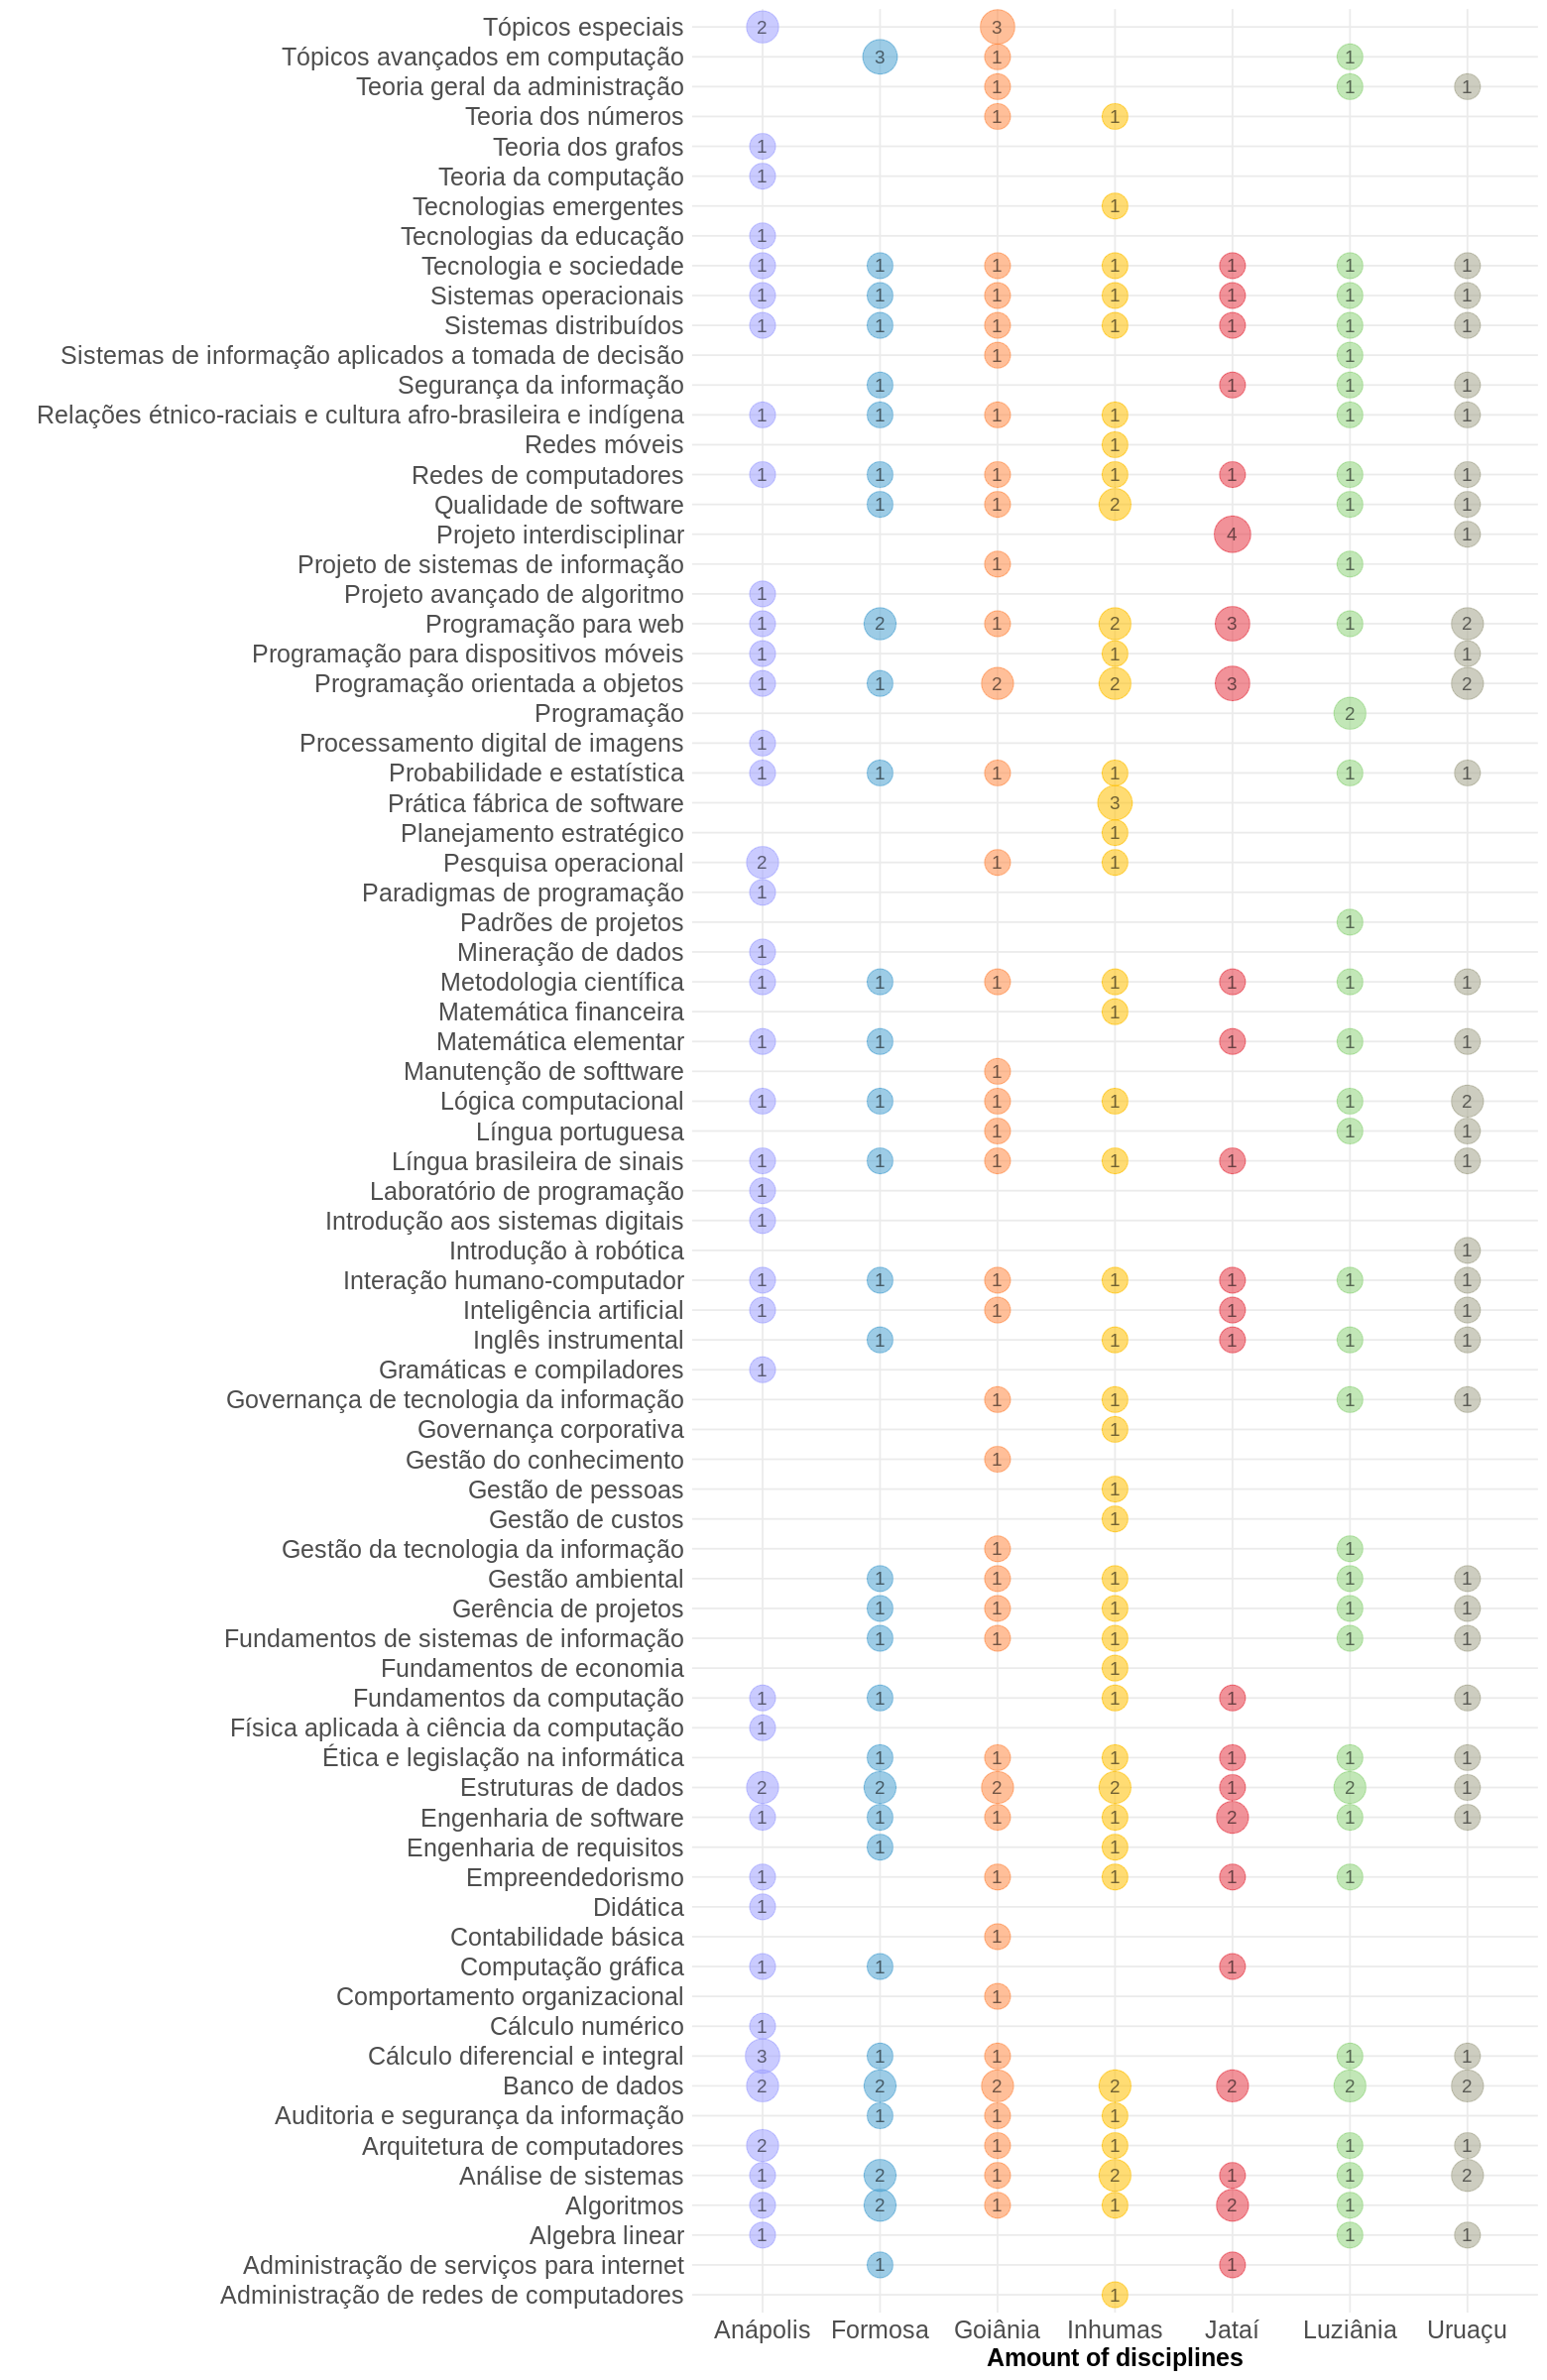
\includegraphics[width=.475\textwidth]{Images/Fig01.png} }}%
    \qquad
    \subfloat[\centering Workload distribution among the themes]{{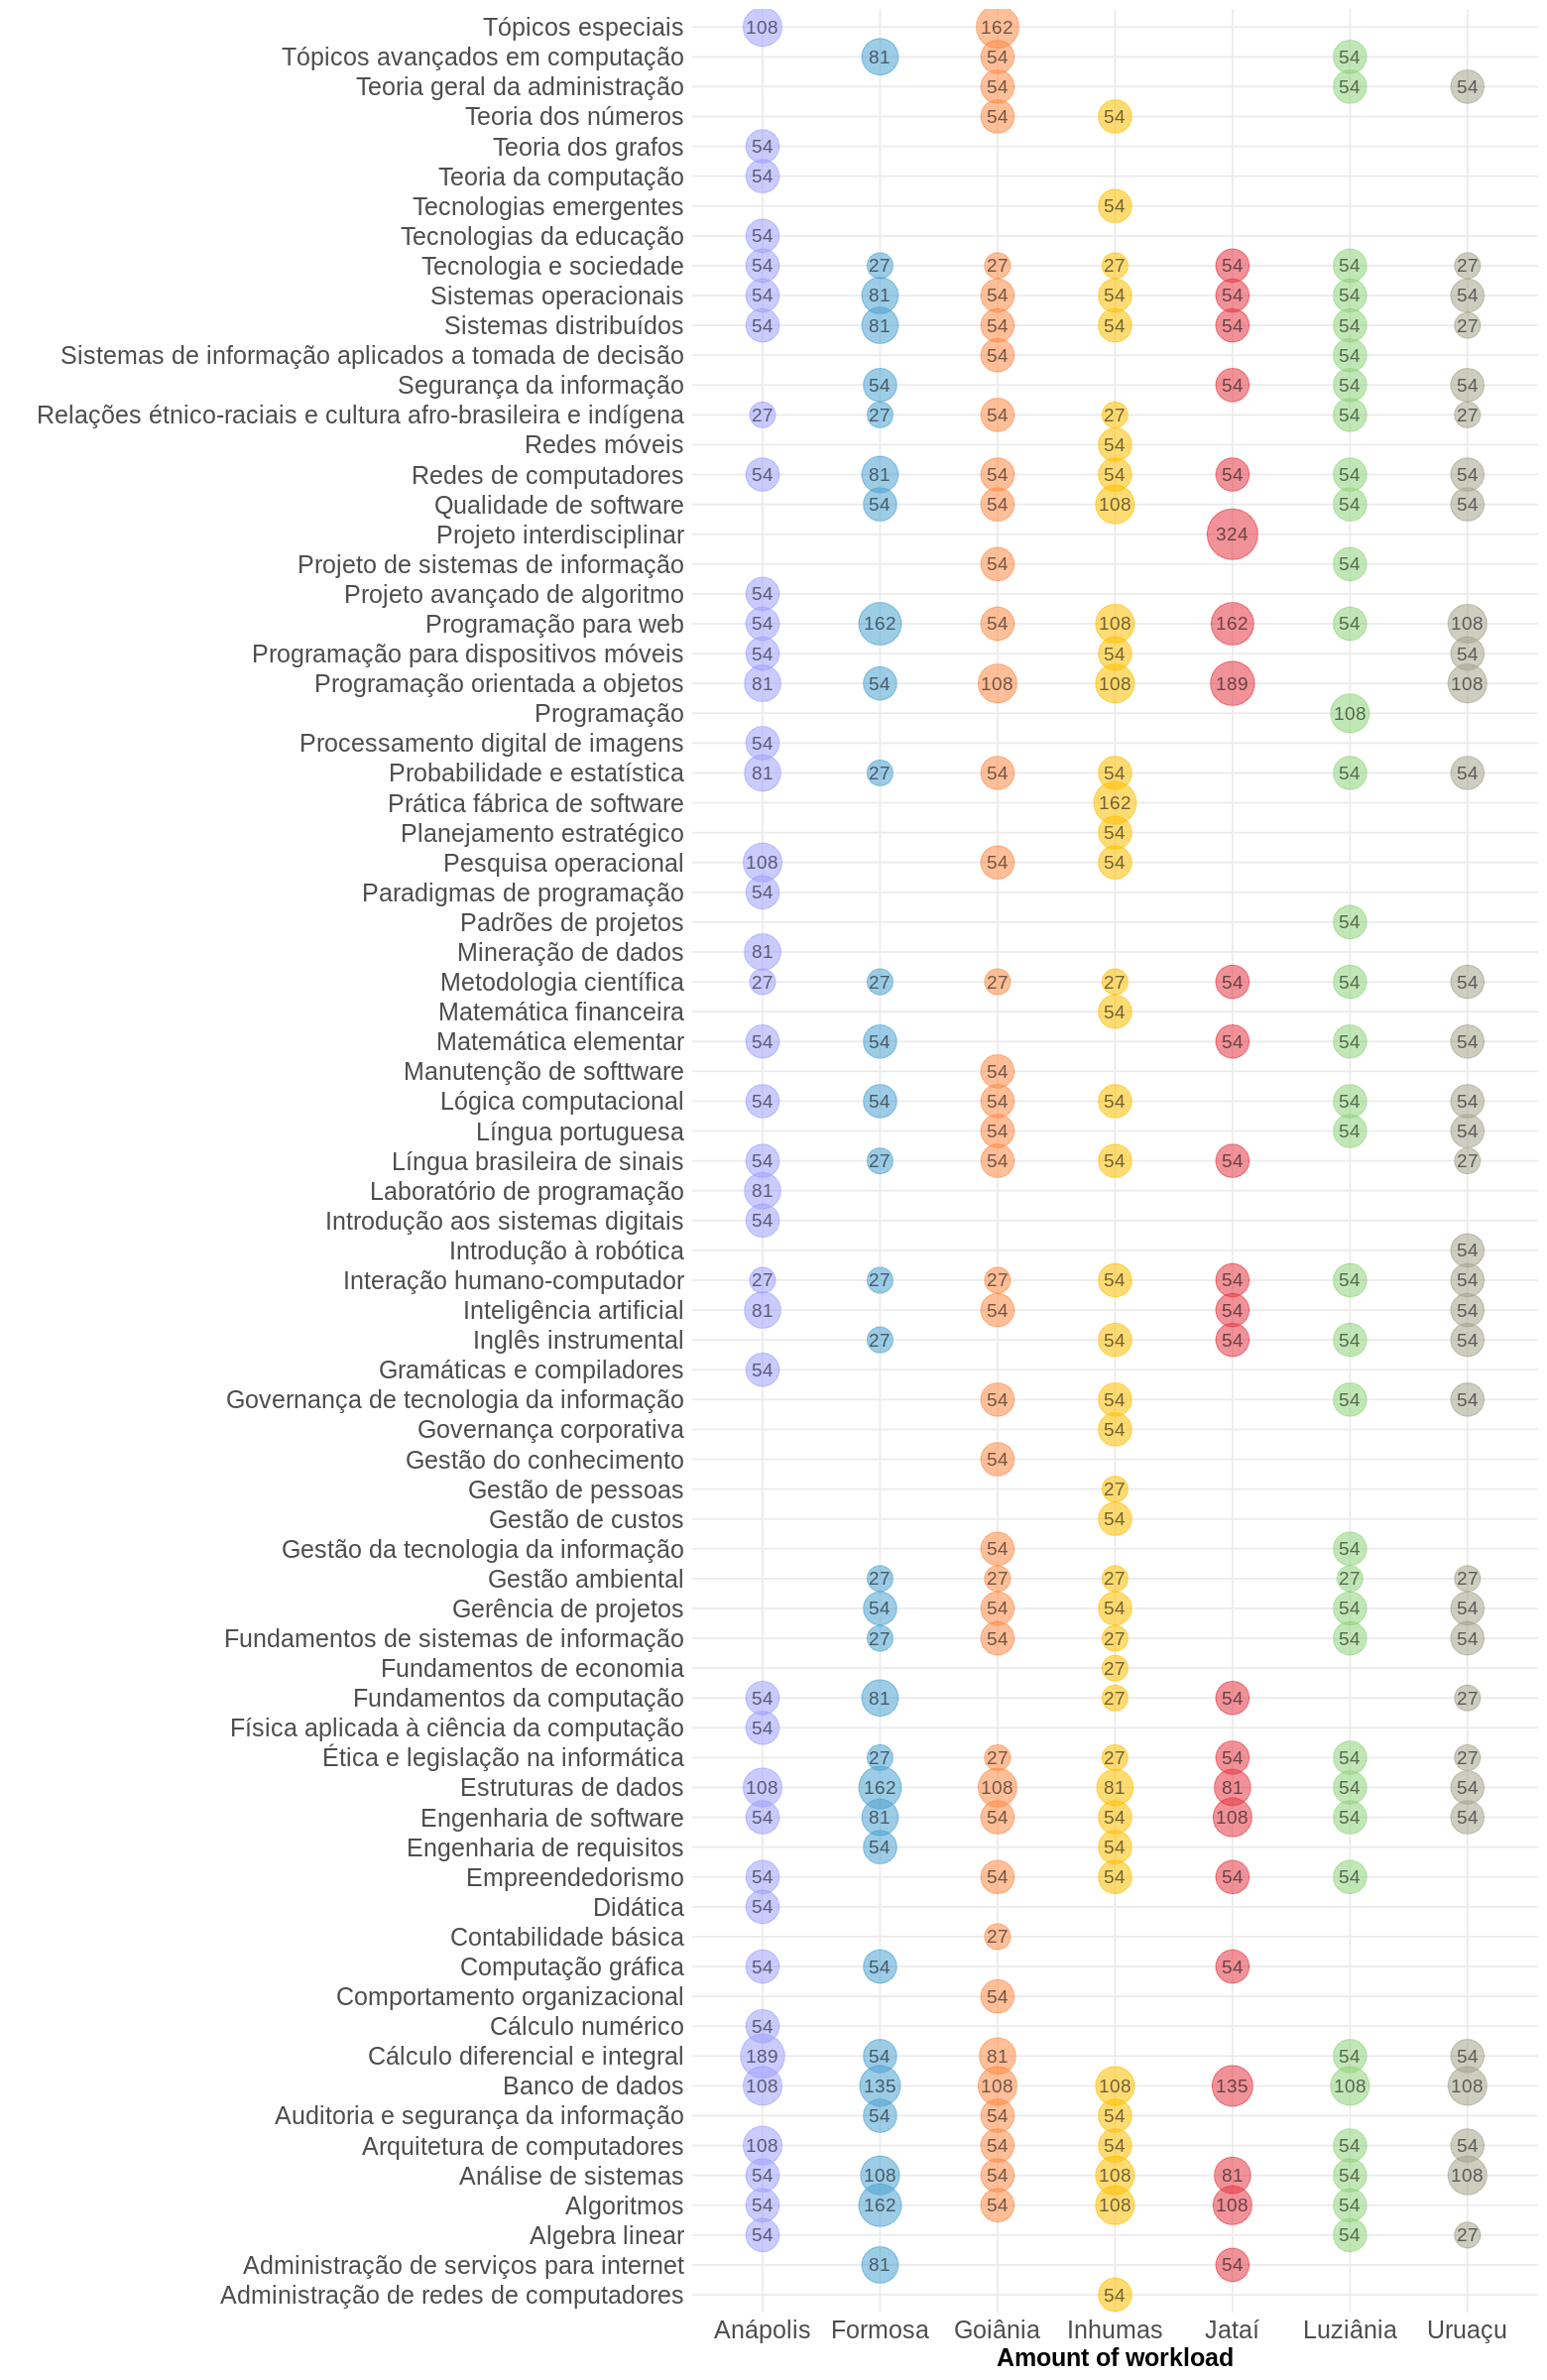
\includegraphics[width=.475\textwidth]{Images/Fig02.png} }}%
    \caption{Themes and disciplines amount (a) and workload (b) distribution among the IFG campuses.}%
    \label{fig_distribution}%
\end{figure*}
~
\begin{figure*}[!htbp]
    \centering
    \subfloat[\centering Amount of disciplines by theme.]{{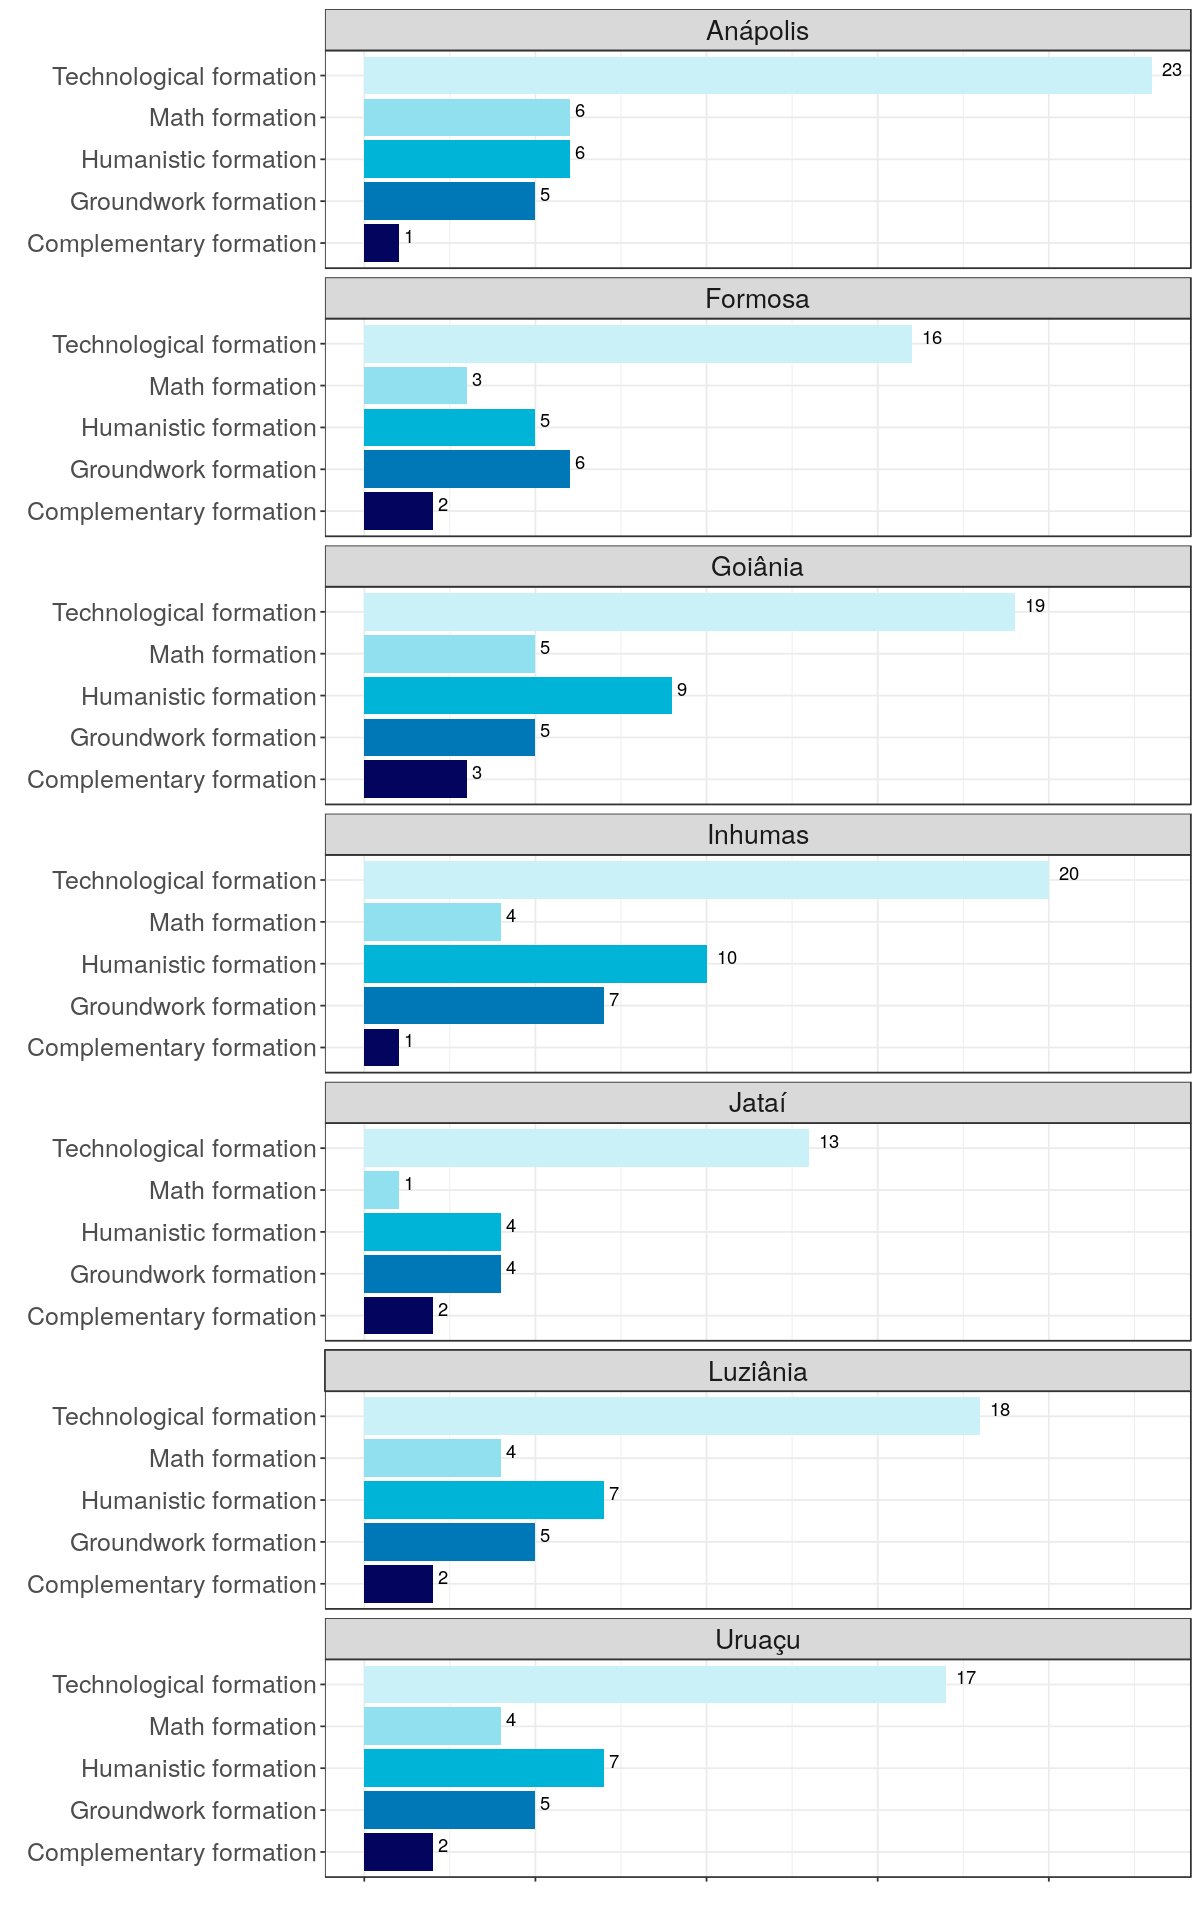
\includegraphics[width=.475\textwidth]{Images/Fig03.png} }}%
    \qquad
    \subfloat[\centering Amount of workload by theme.]{{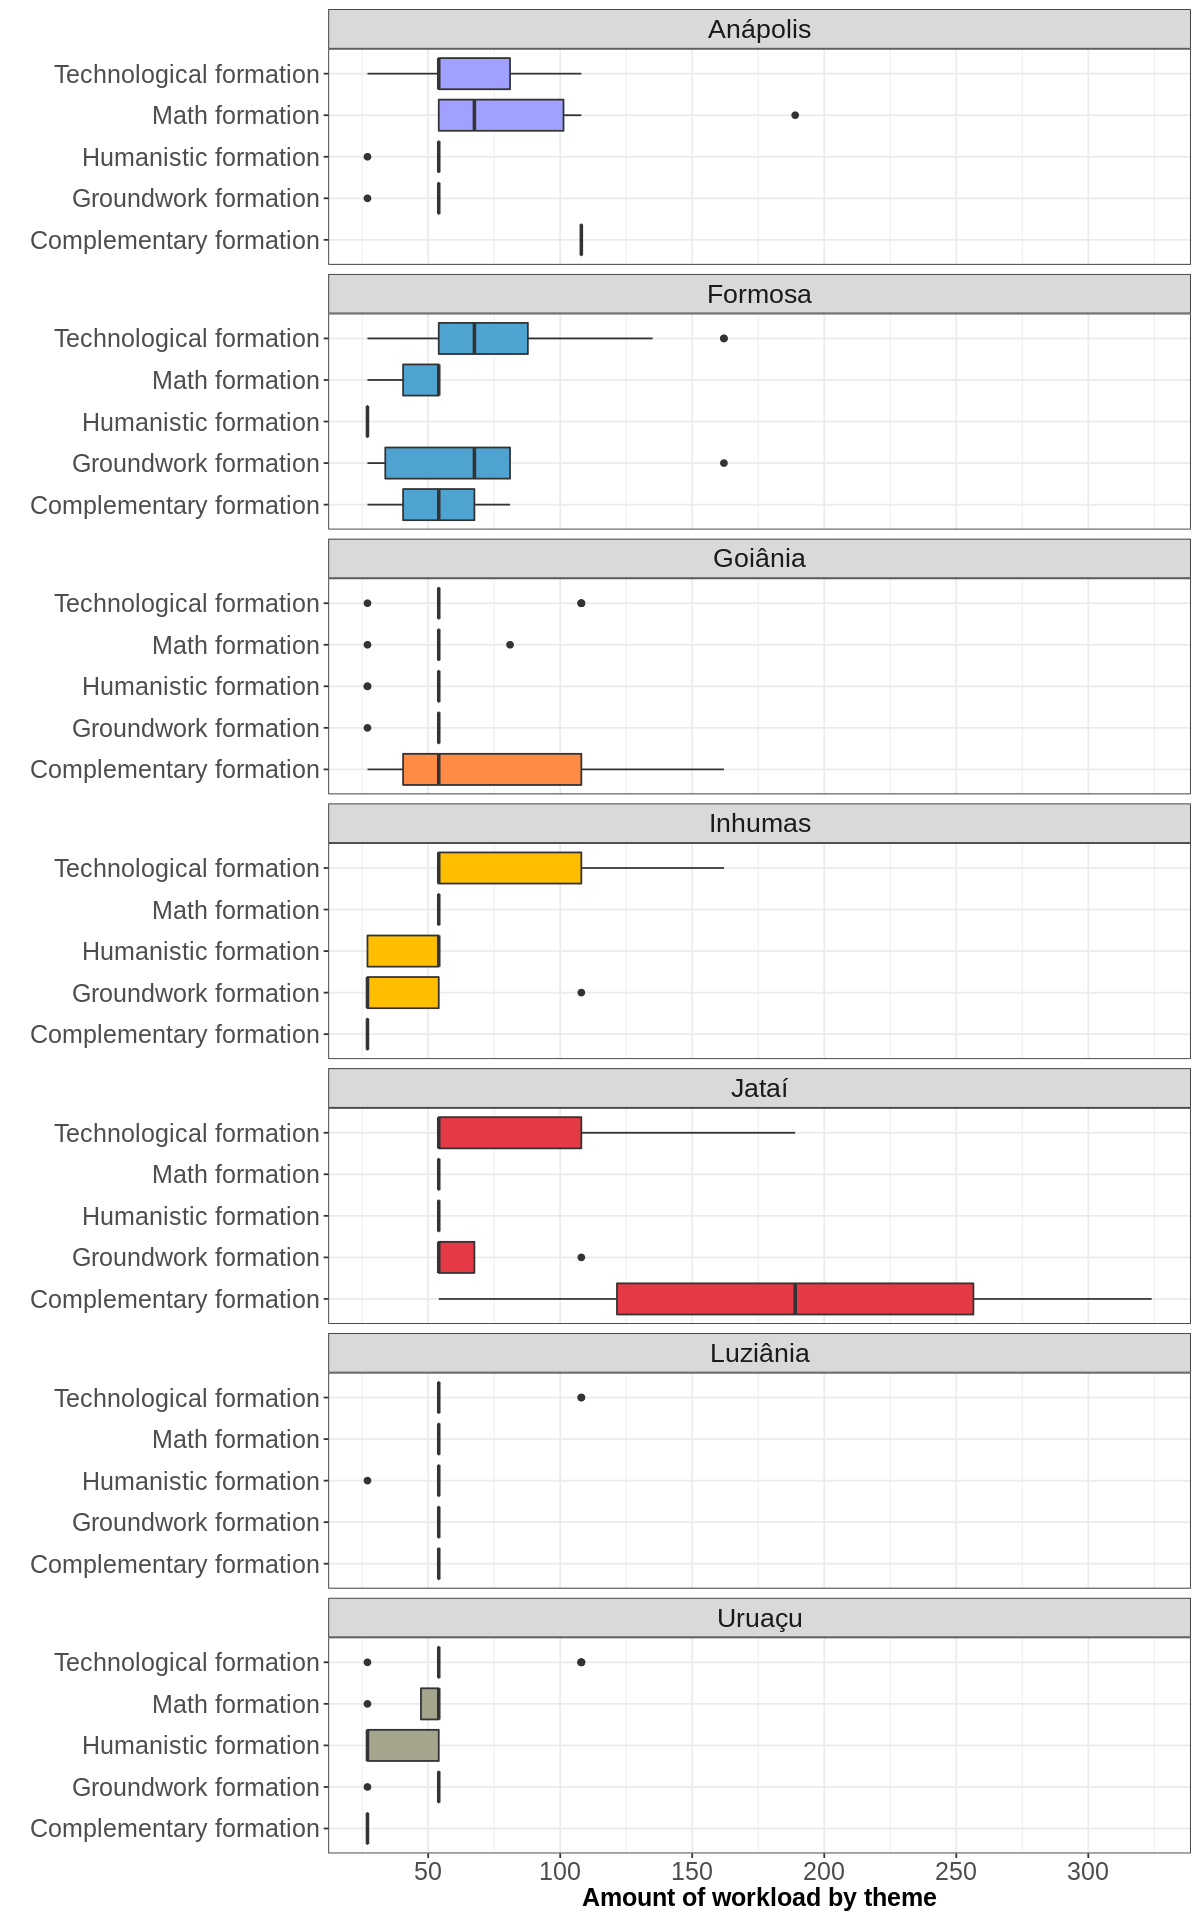
\includegraphics[width=.475\textwidth]{Images/Fig04.png} }}%
    \caption{Amount of disciplines and workload by theme through the IFG campuses.}%
    \label{fig_themes}%
\end{figure*}
The technological formation leads both the workload and the disciplines amount among all the courses.
Math formation is more present in the Bachelor in Computer Science (Anápolis) but closely followed by other courses, except for the courses on Analysis and Development of Systems in Formosa and Jataí, the latter with the minor workload in this theme.
The humanistic formation stands out in Bachelor of Information Systems courses in Goiânia, Inhumas, and Luziânia, but also in the Analysis and Development of Systems in Uruaçu.
Groundwork formation and complementary formation are balanced in all courses, except for the Bachelor in Computer Science course in Anápolis, with only one discipline for complementary formation.
The highlights in math formation at the Bachelor in Computer Science (Anápolis) and humanistic formation at the Bachelors of Information Systems (Goiânia, Inhumas, and Luziânia) are expected, given the nature of these courses.
If considering the workload (\ref{fig_themes}b) over the number of disciplines, the math formation is also more significant in Bachelor in Computer Science course in Anápolis.
The workload for groundwork formation is relatively uniform except for some variation in Analysis and Development of Systems (Formosa) and Bachelors of Information Systems (Inhumas).
The humanistic formation workload is also nearly uniform except for the Analysis and Development of Systems in Formosa.
The most notable distortion is on the complementary formation in the Analysis and Development of Systems of Jataí due to the interdisciplinary projects.

We have proposed ten specific characteristics that we consider essential in a course curriculum, and we check for their presence or absence in the IFG course curriculum.
The result of this analysis is shown in Table~\ref{tab_features}.
\begin{table*}[htbp]
\centering
\caption{Proposed essential features for IFG's Computer Science-related curricula.}
\label{tab_features}
\resizebox{\textwidth}{!}{%
\begin{tabular}{@{}llllllll@{}}
\toprule
\textbf{Feature} & \textbf{Anápolis} & \textbf{Goiânia} & \textbf{Inhumas} & \textbf{Luziânia} & \textbf{Formosa} & \textbf{Jataí} & \textbf{Uruaçu} \\ \midrule
Presence of discipline that addresses work relationships with local productive arrangements & Absent & Absent & Absent & Absent & Absent & Absent & Absent \\
Presence of distance learning or blended disciplines & Absent & Absent & Absent & Absent & Present & Present & Present \\
Presence of disciplines that address Environmental Education & Present & Present & Present & Present & Present & Present & Present \\
Presence of discipline that addresses ethnic/sociocultural diversity & Present & Present & Present & Present & Present & Present & Present \\
The curriculum meets the criteria and recommendations of the SBC Curriculum Reference. & Present & Present & Present & Present & Present & Present & Present \\
The curriculum meets the criteria and recommendations of the Legal Basis (Resolutions and DCNs) & Present & Present & Present & Present & Present & Present & Present \\
The workload curriculum prioritizes Technological/Specific Training disciplines & Absent & Present & Present & Present & Present & Present & Present \\
Complementary training in the Management Area & Present & Present & Present & Present & Present & Present & Present \\
Formation in Mathematics & Present & Present & Present & Present & Present & Present & Present \\
Strong computer science formation & Present & Absent & Absent & Absent & Absent & Absent & Absent \\ \bottomrule
\end{tabular}%
}
\end{table*}


\begin{figure*}[!htbp]
    \centering
    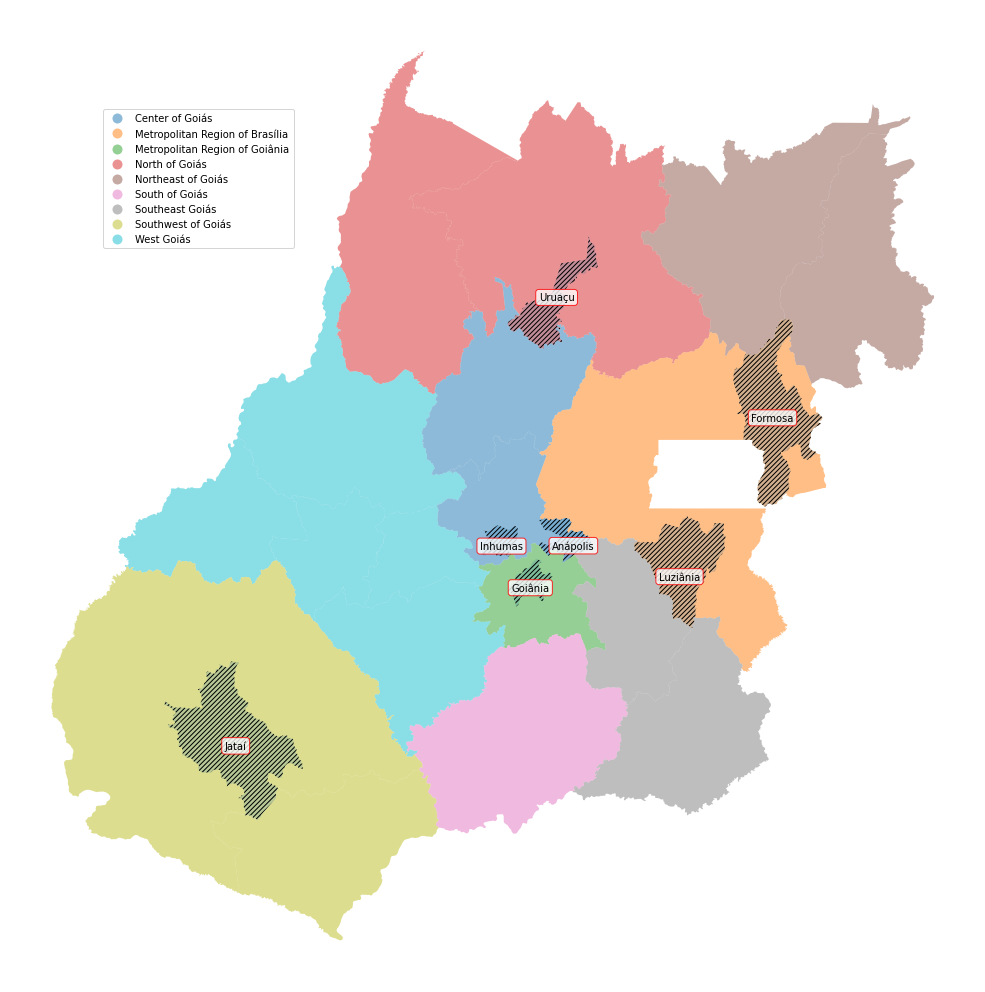
\includegraphics[width=.9\linewidth]{Images/Map.png}%
    \caption{A caption.}
    \label{fig_map}%
\end{figure*}

In 2018, the Goiás government produced the ``Goiás Integrated Economic Development Plan 2038 (PDEIG-2038)''~\cite{goias2038}.
This document contains assumptions and development proposals for the state of Goiás, considering the period between 2018 and 2038.
The document situates the state of Goiás in the Brazilian scenario and presents, among other data, regional trends and vocations to achieve some purposes.
These purposes are related to prosperity, quality of life, public sector efficiency, investor confidence, and leading role in the national scenario.
The Brazilian Institute of Geography and Statistics (IBGE)~\cite{ibge2020} organizes the state of Goiás into regions by grouping characteristics.
One of these groups resulted in nine microregions: Center of Goiás, Metropolitan Region of Brasília, Metropolitan Region of Goiânia, North of Goiás, Northeast of Goiás, South of Goiás, Southeast of Goiás, Southwest of Goiás and West Goiás.
The PDEIG-2038 establishes opportunities according to the type of economic activity in the microregions of Goiás~\cite{ibge2020}.
% Escrever a vocação de cada microregião.

% Estabelecer a relação entre as microregiões e a oferta de computacao do IFG.

% Discutir o impacto do curriculo para a região, para o Brasil e para o mundo.


According to the PDEIG-2038~\citep{goias2038}, the vocations of the northern region of Goiás are related to logistical infrastructure for national integration, ecological and adventure tourism, environmental services, mineral processing, integration of crops, livestock, and forestry.
The Uruaçu campus is located in this region (see Figure~\ref{fig_map}), offering the TADS course.
The computer science area can permeate all these areas as middleware, but some specialized knowledge would be necessary to bridge them.
Such complementary knowledge is not a robust asset in this curriculum.
In the metropolitan region of Brasília (see Figure~\ref{fig_map}), the Formosa and luziânia campuses offer a TADS and a BSI course, respectively. 
The vocation for this area is related to irrigated agriculture, modern services, and information technology.
These courses seem to cope with this region's expectations despite most of the demand for information technology services coming from the federal district, a separate region from Goiás, where the capital of Brazil, Brasília, is located.
The curricula of the courses are similar in terms of the number of disciplines and workload in the selected subjects, except for the different nature of the courses, a TADS (Formosa) and a BSI (Luziânia).

The campuses Anápolis and Inhumas offer a Computer Science undergraduate and a BSI, respectively.
These campuses are located in the Center region of Goiás, close to the capital Goiânia.
According to the report, the vocations of this region are diversified, highlighting the pharmaceutical, defense, and beverage industries, logistics, environmental and information technology services, as well as livestock and agriculture.
The curricula of Anápolis and Inhumas courses have the most significant number of disciplines and workloads in the technical area.
The decision to privilege mandatory technical syllabuses leaves an open side in further education, which can be explained by the fact that these courses are in a region with a demand for their core activity.

The metropolitan region of Goiânia has among its leading market exponents the local commerce, the health area, education, and information technology services.
The Goiânia campus offers a BSI course.
The number of disciplines and workload related to the proposed themes balances the technical area and the humanistic and complementary formation.

In jataí (southwest region of Goiás), the TADS course comprises the smallest number of disciplines in the technical area, but still a workload within the average of the others.
The highlight of this course is the complementary training, with interdisciplinary projects with open menus that can provide an opportunity to integrate with the demands of the region.



\section{Final Considerations}\label{FinalConsiderations}

\bibliographystyle{ACM-Reference-Format}
\bibliography{references}

\end{document}